\documentclass[journal,onecolumn]{IEEEtran}
\usepackage[utf8]{inputenc}
\usepackage{fontenc}
\usepackage{graphicx}
\usepackage{geometry}
\usepackage{amsmath}
\usepackage{amssymb}
\title{Orbital Control of Satellite using LQG Regulator}
\author{Ananthapadmanabhan M(EE17BTECH11047), Shivam Khandelwal(EE17BTECH11037, Siddharth(EE17BTECH11018), Yashaswi(EE17BTECH11019), Dileep(EE17BTECH11024),Gunasekhar(EE17BTECH11032),Kushal(EE17BTECH11012)}
\date{May 2019}

\begin{document}

\maketitle
\section{Introduction}
Satellites offer the unique possibility of interconnecting users, regardless of their location or distance, and providing a complete spectrum of telecommunication services regardless of bandwidth requirements . A satellite also needs a guidance system to make sure that it maintains the proper angle in relation to the earth. A satellite is launched into its approximate desired orbit by a large rocket, which may be carrying several satellites at the same time. Once a satellite is launched into a desired orbit, it never remains in this ideal orbit.Therefore a common problem in the operation of satellites is to guide them and position them at a desired orbit. During its motion however, it is influenced by numerous forces of diverse intensities and directions, emanating from different sources. These forces tend to disturb the satellite and put it into orbit other than the desired orbit.
\section{Problem statement}
The main objective of the work is to simulate an orbit of a satellite and apply suitable control schemes using LQG regulation in order to keep it in the desired orbit, irrespective of external influences and resulting perturbations, using the minimum possible fuel consumption.
\section{Derivation of satellite motion}
Assumptions:\\
1.No other celestial bodies considered (only Earth gravitational force considered).\\
2.M$>>$m C.O.G located at center of Earth.\\
3.Satellite always remains in the equatorial plane$=>$2 variables are sufficient to describe its position: r(t) and $\theta$(t).\\
3.The altitude (orientation) of the satellite is kept constant.\\
The orbit of a satellite can be described by two non-linear coupled equations, which are obtained from an application of the fundamental equation of motion (Newton’s 2nd Law). \\
\begin{equation}m(\ddot{r}-r\dot\theta^2)=u_1-\frac{GMm}{r^2}+w1\end{equation}
\begin{equation}m(2\dot{r}\dot\theta+r\ddot\theta)=u2+w2\end{equation}

Notations:\\
R: radius of the Earth [m]\\
M: mass of the Earth [kg]\\
m: mass of the satellite [kg]\\
r(t): distance from Earth center to satellite [m]\\
$\theta$(t): orbit angle of the satellite [rad]\\
G:Universal Gravitation constant\\
$u_{1}$: thrust in the radial direction\\
$u_{2}$: thrust in the tangential direction\\
$w_{1}$:White noise disturbance with variance $\delta_{1}$\\
$w_{2}$:White noise disturbance with variance $\delta_{2}$\\
Note that $w_{1}$ and $w_{2}$ are independent\\
Let,\\
$r=x_{1}$ \hspace{1cm}$\dot r=x_{2}$ \hspace{1cm}$\theta=x_{3}$\hspace{1cm}$\dot\theta=x_{4}$\\
Writing in state space format\\
\begin{equation}
x=\begin{pmatrix}
x_1\\
x_2\\
x_3\\
x_4\\
\end{pmatrix}
\end{equation}
\begin{equation}
\dot{x}=\begin{pmatrix}
x_2\\
x_1x_4^2-\frac{GM}{x_1^2}\\
x_4\\
-2 (\frac{x_2x_4}{x_1})
\end{pmatrix}+\begin{pmatrix}
0&0\\
\frac{1}{m}&0\\
0&0\\
0&\frac{1}{mx_1}
\end{pmatrix}
\begin{pmatrix}
u_1\\
u_2
\end{pmatrix}
+\begin{pmatrix}
0&0\\
\frac{1}{m}&0\\
0&0\\
0&\frac{1}{mx_1}
\end{pmatrix}
\begin{pmatrix}
w_1\\
w_2
\end{pmatrix}\\
\end{equation}

Equilibrium orbit is given by\\
\begin{equation}
x_o=\begin{pmatrix}
r_o\\
0\\
w_{ot}\\
w_o
\end{pmatrix}\\,
u_1_o =\hspace{1} u_2_o = \hspace{1} w_1_o = \hspace{1} w_2_o=0
\end{equation}
Consider,
\begin{equation}
  x=x_o+dx,u_1=u_1_o+du_1,u_2=u_2_o+du_2,w_1=w_1_o+dw_1,w_2=w_2_o+dw_2  
\end{equation}
\begin{equation}
    \dot{x}=\dot{x_o}+\frac{der(\dot{x})}{der(x)}dx+\frac{der(\dot{x})}{der(u)}du+\frac{der(\dot{x})}{der(w)}dw
\end{equation}
\begin{equation}
\frac{der(\dot{x})}{der(x)}dx=\begin{pmatrix}
(1)dx_2\\
(x_4^2+2\frac{GM}{x_1^3})dx_1+(2x_1x_4)dx_4)\\
(1)dx_4\\
(-2\frac{x_4}{x_1})dx_2-2(\frac{x_2}{x_1})dx_4+2(\frac{x_2*x_4}{x_1^2})dx_1)
\end{pmatrix}\\
\end{equation}
\begin{equation}
\frac{der(\dot{x})}{der(x)}dx=\begin{pmatrix}
0&1&0&0\\
x_4^2+2\frac{GM}{x_1^3}&0&0&2x_1x_4\\
0&0&0&1\\
\frac{x_2*x_4}{x_1^2}&-2\frac{x_4}{x_1}&0&-2\frac{x_2}{x_1}
\end{pmatrix}\begin{pmatrix}
dx_1\\
dx_2\\
dx_3\\
dx_4
\end{pmatrix}\\
\end{equation}

Similarly,\\
\begin{equation}
\frac{der(\dot{x})}{der(u)}du=\begin{pmatrix}
0&0\\
\frac{1}{m}&0\\
0&0\\
0&\frac{1}{mr_o}
\end{pmatrix}
\begin{pmatrix}
du_1\\
du_2
\end{pmatrix}
\end{equation}
\begin{equation}
\frac{der(\dot{x})}{der(w)}dw=\begin{pmatrix}
0&0\\
\frac{1}{m}&0\\
0&0\\
0&\frac{1}{mr_o}
\end{pmatrix}
\begin{pmatrix}
dw_1\\
dw_2
\end{pmatrix}
\end{equation}
Also,$u_1_o=u_2_o=w_1_o=w_2_o=\dot{x}_2_o=0$\\
Therefore from equation(1) evaluated at equilibrium points,we have
\begin{equation}
   x_4_o^2=w_o^2=\frac{GM}{x_1^2}=\frac{GM}{r_o^2} 
\end{equation}
Linearized expression of $d\dot{x}$ about equilibrium points\\
\begin{equation}
d\dot{x}=\dot{x}-\dot{x_o}=\begin{pmatrix}
0&1&0&0\\
3w_o^2&0&0&2r_ow_o\\
0&0&0&1\\
0&-2\frac{w_o}{r_o}&0&0
\end{pmatrix}\begin{pmatrix}
dx_1\\
dx_2\\
dx_3\\
dx_4
\end{pmatrix}+\begin{pmatrix}
0&0\\
\frac{1}{m}&0\\
0&0\\
0&\frac{1}{mr_o}
\end{pmatrix}
\begin{pmatrix}
du_1\\
du_2
\end{pmatrix}
+\begin{pmatrix}
0&0\\
\frac{1}{m}&0\\
0&0\\
0&\frac{1}{mr_o}
\end{pmatrix}
\begin{pmatrix}
dw_1\\
dw_2
\end{pmatrix}\\
\end{equation}
\section{Control System Model and Design}

The following figure shows the block diagram of the given problem.
\begin{figure}[h!]
\centering

 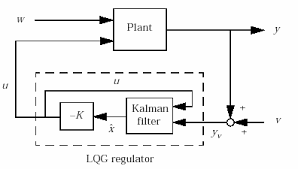
\includegraphics[scale=1.0]{blockdiagram.png}
  \caption{Block Diagram for LQG regulator}
\end{figure}
\\
The above mentioned LQG regulator is achieved through design of gain feedback and Kalman estimator design.
A given LTI system can be modelled as 

\begin{equation}
    \dot x = Ax + B_{u}x + B_{w}w
\end{equation}
\begin{equation}
    y = C_{y}x + D_{yw}w 
    \end{equation}
    \begin{equation}
    z = C_{z}x + D_{zu}u
     \end{equation}

From the above state-space representation the following observer-based controller can be developed as:
\begin{equation}
    \dot {\hat x} = Ax + B_{u}{\hat x} + F({\hat y}-y)
\end{equation}
\begin{equation}
    {\hat y} = C_{y}{\hat x}
    \end{equation}
    \begin{equation}
    u = K{\hat x}
     \end{equation}
\subsection{Design of Gain Feedback}
The design of feedback gain matrix is achievable only if the following conditions are true:\\
1.$(A,B_u)$ is stabilizable\\
2.$w$ is Gaussian zero mean white noise with variance $W\succ0$\\
3. $C^{T}_zD_{zu} = 0$ and  $R\succ0$\\

Then the choice of gain matrix $K$ is obtained by minimizing the cost function:
\begin{equation}
    J = \lim_{t\to\infty} E[{z(t)}^{T}z(t)]
\end{equation}
\begin{equation}
    J = \int_{0}^{\infty} (x^2 x^TQx + u^TRu)dt
\end{equation}
Where Q is state variable weighting matrix and R is control variable weighting matrix.\\

The optimal feedback gain matrix is given by
\begin{equation}
    K^{*} = - R^{-1}{B_u}^TX^*
\end{equation}

Where $X^*$ satisfies algebraic Riccati equation 
\begin{equation}
    A^TX^* + X^*A - X^*B_uR^{-1}{B_u}^TX^* + Q = 0
\end{equation}
\subsection{Design of Kalman Estimator}
We consider the following assumptions
1.$(A,C_y)$ is detectable\\
2.$w$ is Gaussian zero mean white noise with variance $W\succ0$\\
3. $B_wW{D_{zu}}^T = 0$ and  $D_{yw}WD^{T}_{yw}\succ0$

Hence estimator matrix is considered as
\begin{equation}
    F^{*} = - Y*C^T_y(D_{yw}WD^{T}_{yw})^{-1}
\end{equation}
where $Y^*$ satisfies algebraic Riccati equation
\begin{equation}
    AY^* + Y^*A^T - Y*C^T_y(D_{yw}WD^{T}_{yw})^{-1}C_yY^* + B_wW{D_{zu}}^T = 0
\end{equation}

\subsection{Closed Loop System}
The following is the state space representation of the closed loop system design using LQG regulator
\begin{equation}
    \begin{pmatrix}
    \dot x\\
    \dot {\hat x}
    \end{pmatrix}
    =
    \begin{pmatrix}
    A&B_uK\\
    -FC_y&A+B_uK+FC_y
    \end{pmatrix}
     \begin{pmatrix}
    x\\
    {\hat x}
    \end{pmatrix}
    +
     \begin{pmatrix}
    B_w\\
    -FD_{yw}
    \end{pmatrix}
    w
\end{equation}
\begin{equation}
    z = 
       \begin{pmatrix}
    C_z&D_{zu}K
    \end{pmatrix}
    \begin{pmatrix}
    x\\
    {\hat x}
    \end{pmatrix}
\end{equation}




\section{Simulation and Validation Results}

In this section, the above LQG regulator method is applied to the orbital control of the satellite, the effectiveness of which can be demonstrated by mathematical simulation test. Then, the simulation results are described as follows.

\subsection{Simulation}
The initial mass of the satellite,distance from earth, simulation time are 300kg, 300km, 1728000s. Values of Q and R are as follows:
\begin{equation}
Q = 
    \begin{bmatrix}
    1&0&0&0\\
    0&1&0&0\\
    0&0&1&0\\
    0&0&0&1
    \end{bmatrix}
\end{equation}
\begin{equation}
R = 
    \begin{bmatrix}
    10000&0\\
    0&10000
    \end{bmatrix}
\end{equation}

\subsection{Simulation Results}
The simulated output for the original system and closed loop system designed using LQG controller is given in Fig.1.\\
\begin{figure}[h!]
\centering

 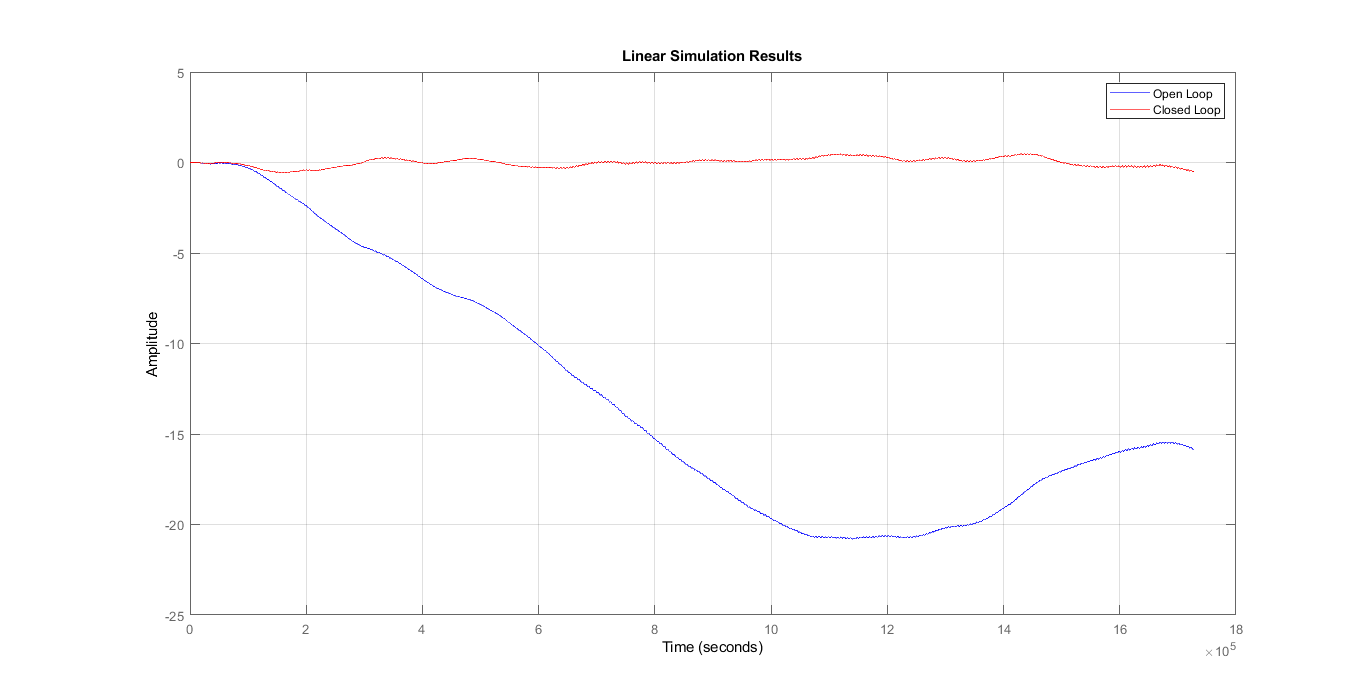
\includegraphics[scale=0.35]{simulation.png}
  \caption{Bode plot(Magnitude) of input $u_1$}
\end{figure}
\\
\\
\\
\\
\\
\\
\\
\\
From the above simulation result, we can see that the deviation due to noise can be controlled within a given boundary.
\\
\\
\\
\\
Fig.2 provides the magnitude of bode plot for the system w.r.t both inputs $u_1$ and $u_2$.


\begin{figure}[h]
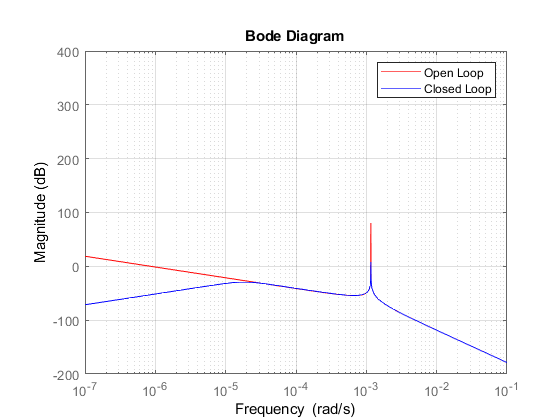
\includegraphics[scale=0.5]{opvsip1.png}
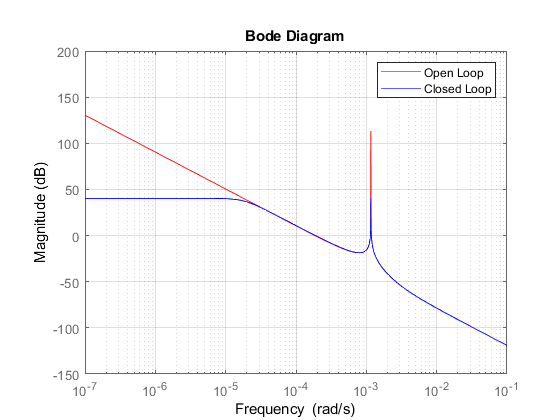
\includegraphics[scale=0.5]{opvsip2.png}
\centering
\caption{Bode plot(Magnitude) of input $u_1$}

\end{figure}

The above fig.2 indicates the attenuation of disturbance effect.
\\
\\
\\
\\
\section{conclusion}
Compared to the conventional methods of to control orbit dynamics the application of LQG regulator provides higher control precision. The method allows to reduce the impact of the external and internal disturbances on the orbital motion of satellite. The above method can be used only for short term and high precision requirements due to higher fuel consumption.
\end{document}
